%%%%%%%%%%%%%%%%%%%%%%%%%%%%%%%%%%%%%%%%%%%%%%%%%%%%%%%%%%%%%%%%%%%%%%%%%%%%%
\section{Dynamic and Irregular Scientific Applications}\label{sec:back-apps}
%%%%%%%%%%%%%%%%%%%%%%%%%%%%%%%%%%%%%%%%%%%%%%%%%%%%%%%%%%%%%%%%%%%%%%%%%%%%%

\subsection{Quantum Monte Carlo Simulation }
\cite{qmcpack}

\subsection{NWChem Quantum Chemistry Application}
NWChem is a widely used quantum chemistry application suite that provides
a large set of simulation capabilities~\cite{nwchem}. Due to the large
memory needs in NWChem that often require memory sharing across multiple
nodes, it is developed based on the Global Arrays toolkit~\cite{GA_SC94}
which provides users with distributed dense arrays that can be accessed
through one-sided operations. Figure~\ref{fig:app-nwchem-pattern}
demonstrates the typical \emp{get-compute-update} pattern used in NWChem.

Current NWChem has been looking at small-to-medium molecules (e.g.,
(H$_2$O)$_{21}$ as shown in Figure~\ref{fig:app-nwchem-w21}) consisting of
20-100 atoms. Since the coulomb interaction among such small amount of
atoms is reasonably large, the computation and communication can be
successful scaled on modern supercomputers. However, scientists aim to
study more complex molecules that are composed of thousands atoms or even
larger thus not only the short-range interactions but also the long-range
interactions have to be covered. This means, the diversity of the amount
of computation per process can be considerably increased, thus resulting
in extremely irregular computation with data movement.

\begin{figure}[h]
\centering
\subfigure[Interaction in (H$_2$O)$_{21}$ molecule.] {
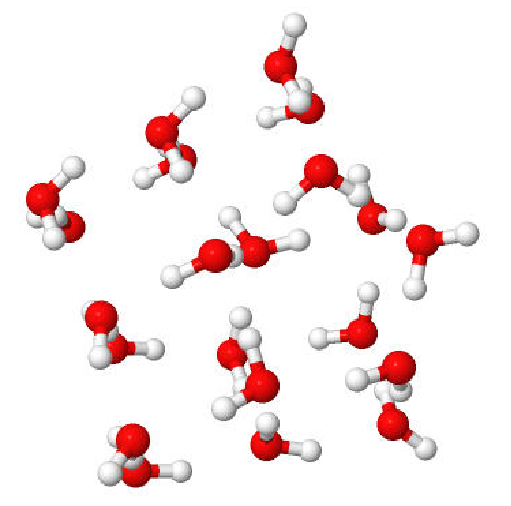
\includegraphics[width=0.38\textwidth]{figures/background/app-nwchem-w21.pdf}
\label{fig:app-nwchem-w21}}
\subfigure[Get-Compute-Update pattern.] {
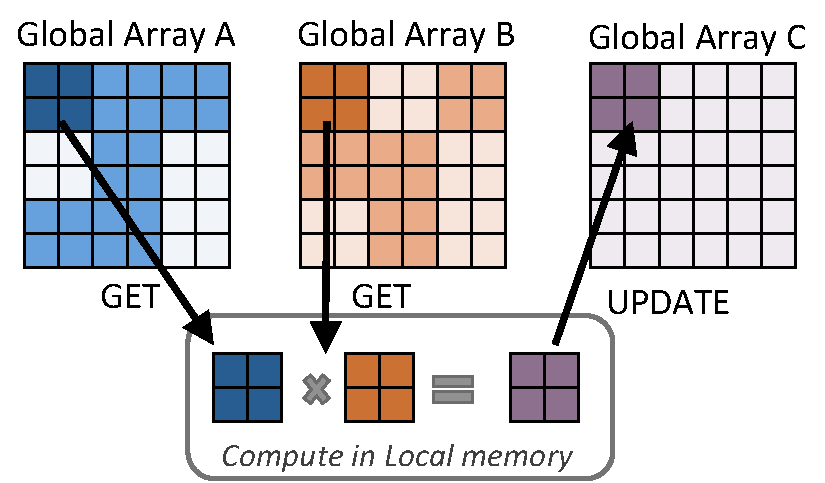
\includegraphics[width=0.56\textwidth]{figures/background/app-nwchem-get-comp-update.pdf}
\label{fig:app-nwchem-pattern}}
\caption{Communication in NWChem Application.}
\label{fig:app-nwchem}
% \vspace{-2.0ex}
\end{figure}


\subsection{SWAP-Assembly Bionformatics Application}

In bioinformatics, since it is still hard to read the whole genomes
in modern DNA sequencing technology, researchers often break down long
DNA samples into large amount of small fragments, called ``reads'', and
then read those reads into digital data as the first step. The next step
is called assembly, which merges overlapping reads back to one or several contiguous DNA sequences. The sequence assembly technology helps biology
scientists analyze DNA sequence, and is especially important for understanding complex environments containing many different microbiomes
(e.g., soil and seawater).

The SWAP-Assembler software provides highly scalable assembler that processes
the sequence assembly on thousands of cores in parallel~\cite{swap}. The
initial reads are represented as a distributed De Bruijn graph (e.g., )
Figure~\ref{fig:app-swap-graph}), and final contiguous DNA chains are
assembled by executing multiple rounds of graph reduction and error removal
over MPI communication. The communication pattern follows the
\emp{send-merge-return} mode as shown in Figure~\ref{fig:app-swap-merge}.
Every process issues each of its local DNA read to a remote process to find
the overlapping reads. On the remote process, it first searches the
overlapping read for every received message, then merges the reads and
finally returns the merged result. If there is no matching read on the
remote side, the sending process will try another remote process following
the same patter. This processing always involves enormous irregular data
movement over petabytes of data and requires several days or even months of
computation. For instance, the largest simulation done to date was at the
University of Chicago, where a 2.3-terabyte sample was assembled on a
supercomputer with 18,000 cores—this simulation took 4 days to complete and
spent 99.9\% of its time idling, because of imbalance between processing
units.


% Reconstruct long DNA sequences by merging many small fragments as shown
% in Figure~\ref{fig:app-swap}.

\begin{figure}
\centering
\subfigure[Graph Reduction.] {
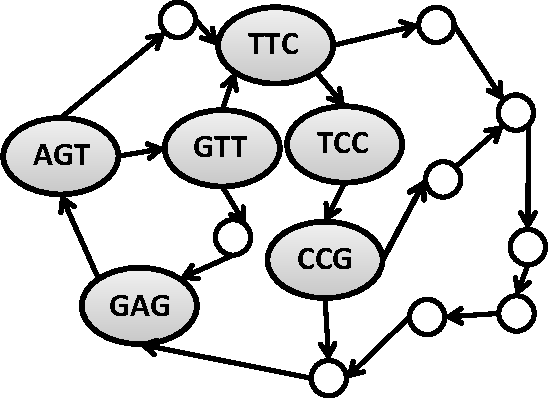
\includegraphics[width=0.3\textwidth]{figures/background/app-swap-graph.pdf}
\label{fig:app-swap-graph}}
\subfigure[Communication Pattern.] {
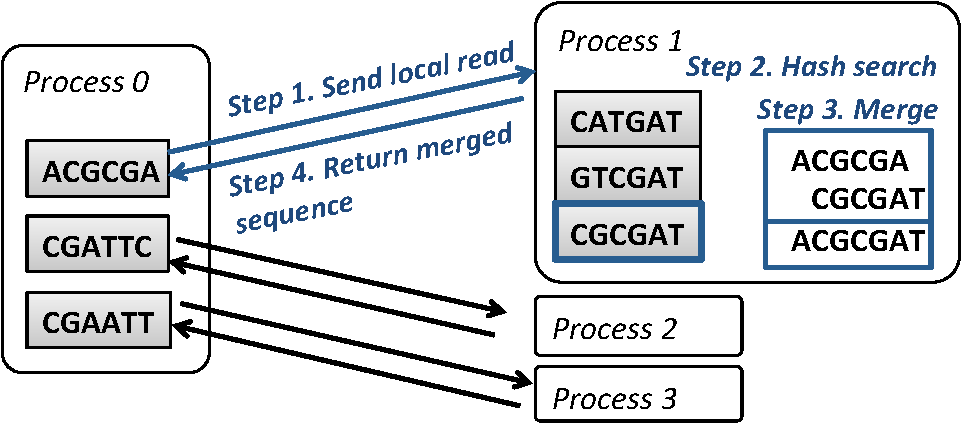
\includegraphics[width=0.65\textwidth]{figures/background/app-swap-merge.pdf}
\label{fig:app-swap-merge}}
% \includegraphics[width=0.9\columnwidth]{figures/background/swap-merge.pdf}
\caption{Irregular Communication in SWAP-Assembly.}
\label{fig:app-swap}
% \vspace{-2.0ex}
\end{figure}

\subsection{Nuclear Reactor Core Modeling}
% \subsection{Green’s Function Monte Carlo}
% \subsection{Graph-Type Parallel Visualization}
